\section{Method}
\label{sec:method}
We present a pipeline for inverse food fracture parameter estimation from a non-differentiable simulator. The pipeline consists of four components: simulation and dataset generation (Sec.~\ref{sec:simulation}), behavioral feature extraction and surrogate modeling (Sec.~\ref{sec:surrogate}), latent space models for parameter compression (Sec.~\ref{sec:latent}), and optimization methods including a goal-conditioned policy and warm-start hybrid (Sec.~\ref{sec:gc}--\ref{sec:warmstart}). Figure~\ref{fig:pipeline} provides an overview.

\begin{figure*}
    \centering
    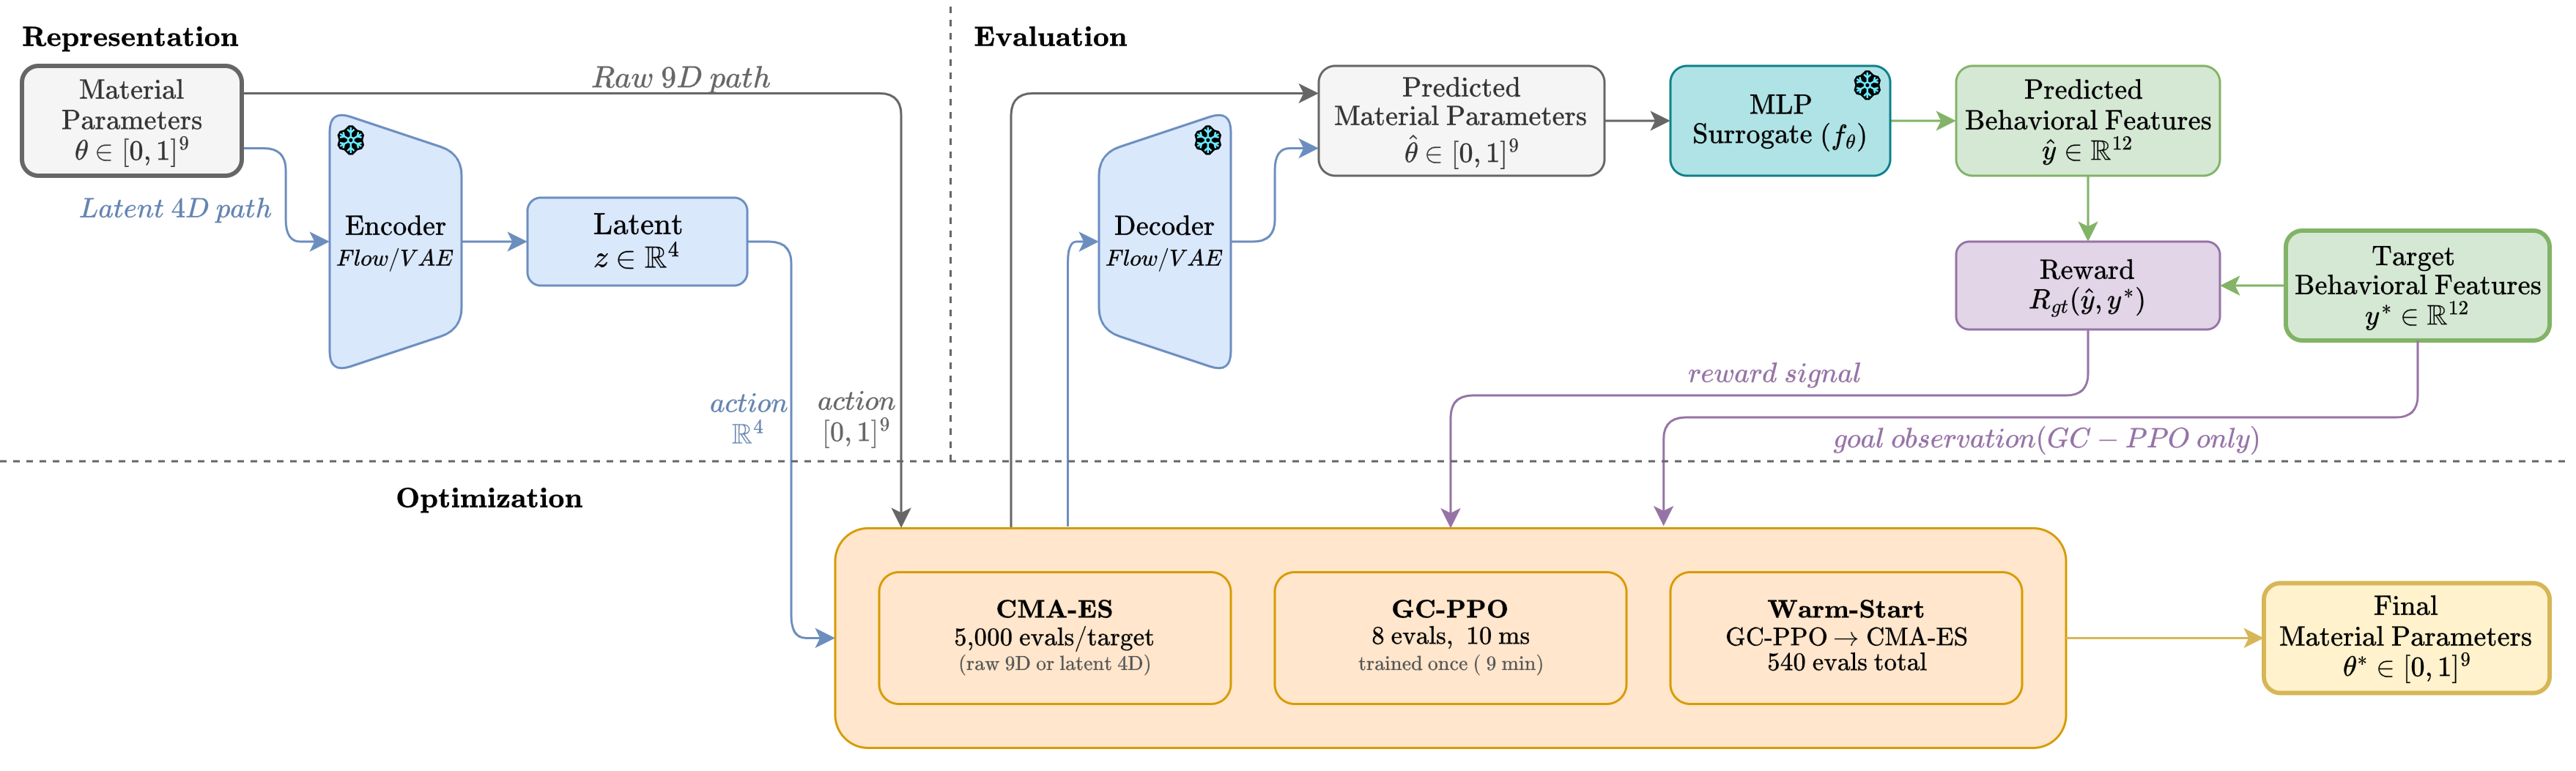
\includegraphics[width=1.0\linewidth]{media/pipeline.png}
    \caption{Method overview. At inference, all pretrained components (encoder, decoder, surrogate) are frozen. \textbf{Representation} (top left): parameters are optimized directly or compressed to a $4$D latent code. \textbf{Optimization} (bottom): CMA-ES searches per-target; GC-PPO conditions on target features $\mathbf{y}^*$ as a goal observation and generalizes across targets; warm-start combines both. \textbf{Evaluation} (top right): proposals are decoded to parameters, passed through the frozen MLP surrogate ($R^2{=}0.937$), and scored against the target. The decode-then-evaluate design ensures all methods use the same evaluator, isolating representation quality from surrogate quality.}
    \label{fig:pipeline}
\end{figure*}


\subsection{Simulation and Parameter Space}
\label{sec:simulation}

We use AnisoMPM~\cite{wolper2020anisompm} to model orange peeling. AnisoMPM extends MPM~\cite{wolper2019cdmpm} with anisotropic damage mechanics and directional fiber reinforcement, necessary because orange skin exhibits directional fiber structure that resists tearing preferentially along certain orientations. Standard isotropic MPM cannot capture this behavior. The simulation represents an orange half with distinct skin and interior (flesh) material regions, where a gripper pulls the skin away from the interior along a fixed arc trajectory (Figure~\ref{fig:sim_scene}). The skin is modeled with anisotropic fiber reinforcement controlled by the fiber stiffness scale $f_s$. The interior uses isotropic damage mechanics with no fiber reinforcement, representing the softer flesh. Each simulation produces $240$ frames of ${\sim}50{,}000$ particles and runs for ${\sim}156$\,s on $8$ CPU threads.

\begin{figure}[t]
\centering
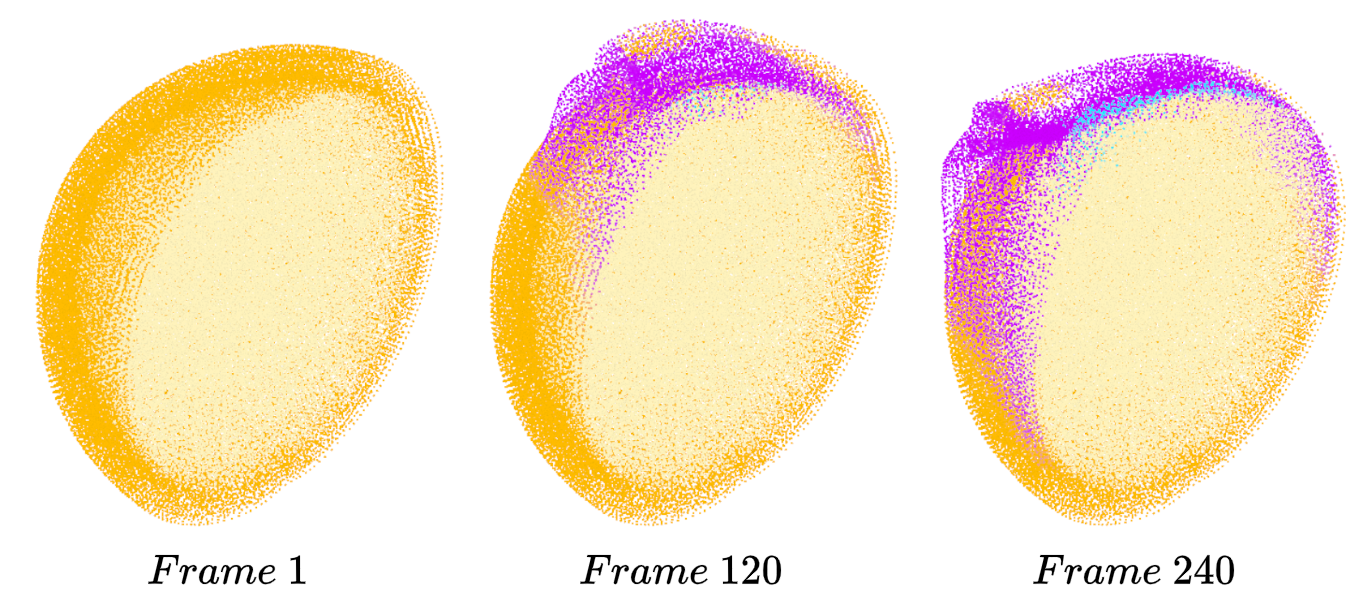
\includegraphics[width=1.0\linewidth]{media/simulation.png}
\caption{AnisoMPM simulation of orange peeling at three stages. Particles are colored by region and damage: orange (intact skin), yellow (intact flesh), purple (damaged skin), cyan (damaged flesh). The anisotropic fiber-reinforced skin resists tearing along preferred orientations, producing heterogeneous fracture patterns that depend sensitively on the $9$ material parameters (Table~\ref{tab:params}).}
\label{fig:sim_scene}
\end{figure}

The simulation is controlled by 9 physical parameters (Table~\ref{tab:params}). Two parameters are shared across regions: Young's modulus $E$ and density $\rho$. Each region has independent fracture threshold $\sigma$, damage regularization $\eta$, and residual stress $r$. The skin additionally has a fiber stiffness scale $f_s$ controlling anisotropic reinforcement along material fibers. All parameters are normalized to $[0,1]$ for optimization, with log-scale transformation for the six that span multiple orders of magnitude.

\begin{table}[t]
\centering
\caption{The 9 material parameters, with physical ranges and region assignments. Six parameters (marked $\dagger$) use log-scale normalization.}
\label{tab:params}
\small
\begin{tabular}{lccc}
\toprule
\textbf{Parameter} & \textbf{Symbol} & \textbf{Range} & \textbf{Region} \\
\midrule
Young's modulus$^\dagger$ (Pa) & $E$ & $[50, 8000]$ & shared \\
Density               & $\rho$ & $[0.5, 10]$ & shared \\
Fracture threshold    & $\sigma_{\text{s}}$ & $[0.05, 0.5]$ & skin \\
Damage regularization$^\dagger$ & $\eta_{\text{s}}$ & $[0.01, 1.0]$ & skin \\
Residual stress$^\dagger$       & $r_{\text{s}}$ & $[0.001, 0.1]$ & skin \\
Fiber stiffness$^\dagger$       & $f_s$ & $[1, 100]$ & skin \\
Fracture threshold    & $\sigma_{\text{i}}$ & $[0.1, 0.9]$ & interior \\
Damage regularization$^\dagger$ & $\eta_{\text{i}}$ & $[0.01, 1.0]$ & interior \\
Residual stress$^\dagger$       & $r_{\text{i}}$ & $[0.001, 0.1]$ & interior \\
\bottomrule
\end{tabular}
\end{table}

We generate $N = 2{,}000$ simulations by sampling material parameters uniformly across the normalized parameter space, totaling $87$ hours of compute. The simulator is deterministic (verified with zero variance across $5$ identical runs), so any discrepancy between surrogate-predicted and simulator-validated rewards is attributable entirely to surrogate inaccuracy.

\subsection{Feature Extraction and Neural Surrogate}
\label{sec:surrogate}
Running the simulator is too expensive for direct use in optimization ($2.6$ minutes per evaluation). We address this by defining a compact set of behavioral features that summarize each simulation's outcome, then training a fast neural surrogate that predicts these features from material parameters.

% For each simulation, we extract $12$ aggregate behavioral features that capture macroscopic peeling characteristics. The extractor reads every 10th frame (yielding ${\sim}24$ frames from $240$), splitting particles into skin and interior groups using a per-particle label. Features include skin-to-interior centroid separation distance, peak separation rate, fracture onset frame, skin dispersion and detachment fraction, interior displacement statistics, interior dispersion, mean phase- field damage in each region, and the interpolated frame at which separation reaches half its final value.

We design $12$ aggregate behavioral features that capture macroscopic peeling characteristics. These features are hand-crafted from domain knowledge of the peeling process and computed from the raw particle data by reading every 10th frame (yielding ${\sim}24$ frames from $240$) and splitting particles into skin and interior groups using a per-particle label stored in the simulation output. The features capture four aspects of peeling behavior: separation dynamics (final centroid distance between skin and interior, peak separation rate, fracture onset frame, separation half-time), skin behavior (spatial dispersion, detachment fraction), interior behavior (mean and maximum displacement, spatial dispersion), and material damage (mean damage scalar in skin and interior regions).

We train an MLP surrogate $f_\theta: [0,1]^9 \to \mathbb{R}^{12}$ predicting features from parameters (Figure~\ref{fig:training}a). The architecture is a multi-layer perceptron with hidden dimensions ($256$, $256$, $128$), a skip connection concatenating the outputs of the first two layers into a $512$-dimensional input to the third, batch normalization, ReLU activations, and dropout ($0.1$). Training uses MSE loss on standardized features with an 80/20 split ($1{,}600$ / $400$ samples), Adam optimizer (learning rate $10^{-3}$, weight decay $10^{-4}$), and early stopping with patience $50$. The surrogate achieves $R^2 = 0.937$ overall (per-feature range: $0.854$ to $0.991$) and evaluates in ${\sim}0.1$\,ms, a $1.5 \times 10^6$ speedup over the simulator.

\paragraph{Reward function.}
We define a recovery reward measuring how well predicted features match a target:
\begin{equation}
    R_{\text{gt}}(\mathbf{y}, \mathbf{y}^*) = \exp\!\Biggl(-\kappa\sqrt{\frac{1}{M}\sum_{k=1}^{M} \biggl(\frac{y_k - y^*_k}{s_k}\biggr)^{\!2}}\;\Biggr),
\label{eq:gt_reward}
\end{equation}
where $\mathbf{y}^*$ is the target feature vector, $s_k = p_{95,k} - p_{5,k}$ is the percentile-based scale from the dataset, $M{=}12$ is the number of features, and $\kappa{=}3$ controls the sharpness of the reward around the target. A value of $R_{\text{gt}}{=}1$ indicates perfect feature matching.

\begin{figure*}
\centering
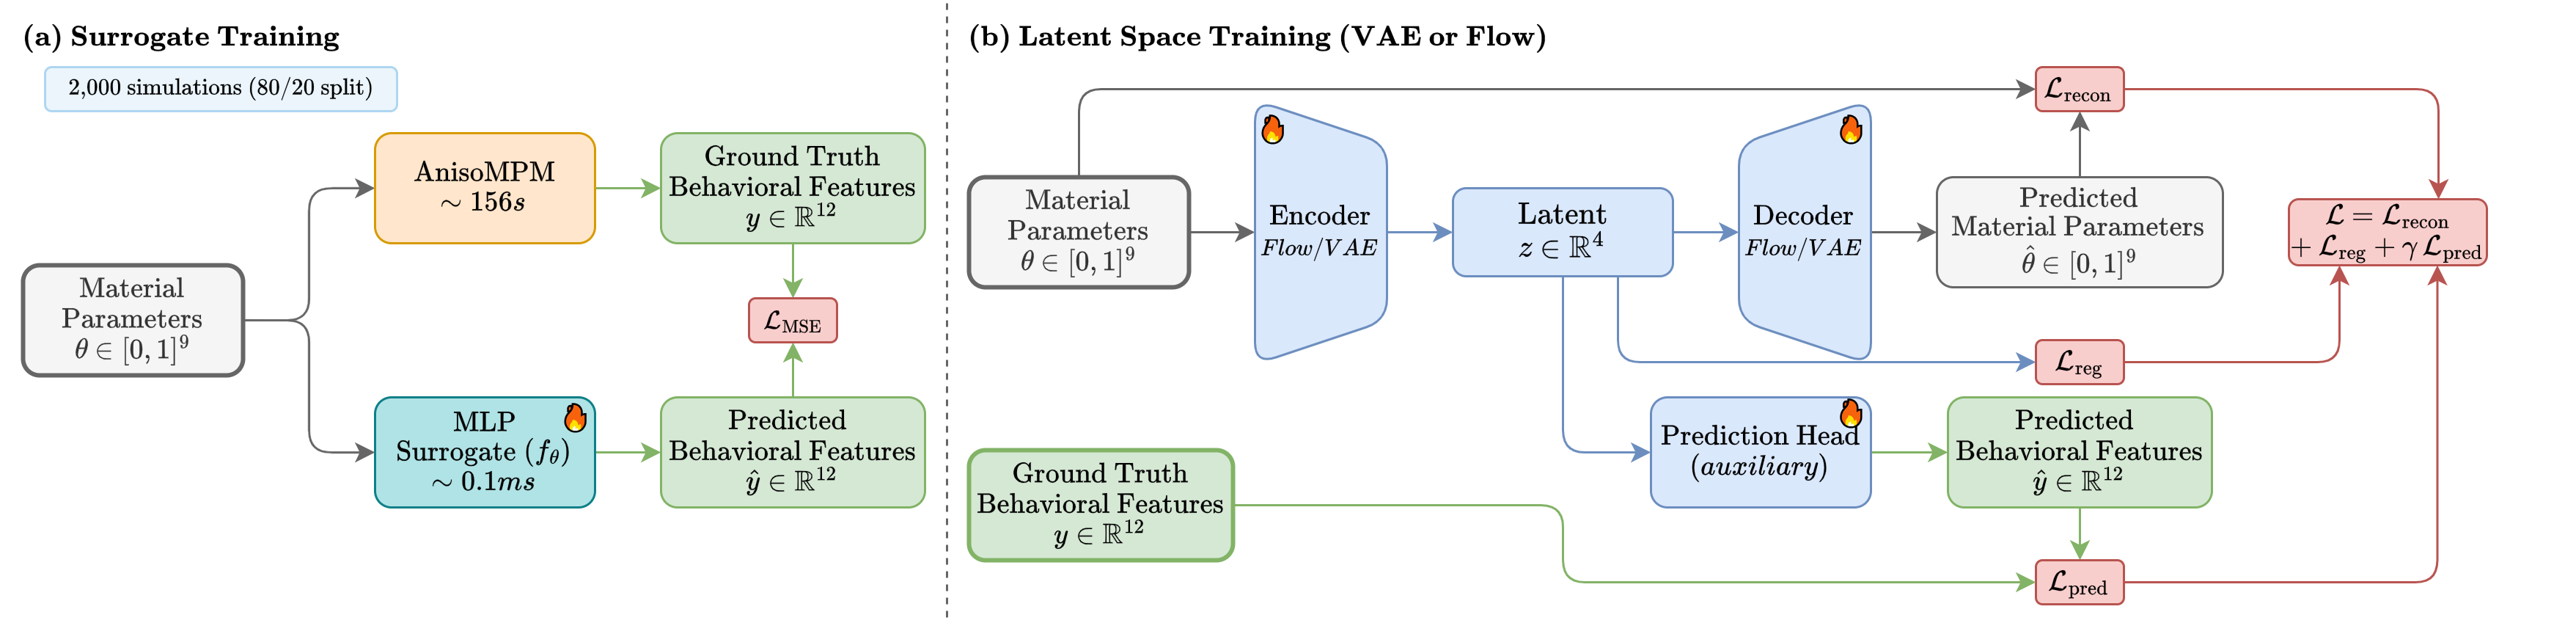
\includegraphics[width=1.0\linewidth]{media/training.png}
\caption{Offline training (trainable modules indicated in figure). \textbf{(a)}~The MLP surrogate learns to predict behavioral features from material parameters, providing a $1.5{\times}10^6$ speedup over the simulator. \textbf{(b)}~The latent model (VAE or flow) compresses the $9$D parameter space to $4$D via three jointly trained objectives: parameter reconstruction ($\mathcal{L}_{\text{recon}}$), latent regularization ($\mathcal{L}_{\text{reg}}$), and behavioral feature prediction ($\mathcal{L}_{\text{pred}}$) via an auxiliary head. The feature prediction term organizes the latent space so that nearby codes produce similar peeling behaviors, enabling efficient RL navigation.}
\label{fig:training}
\end{figure*}

\subsection{Latent Space Models}
\label{sec:latent}

We compare two generative models that compress the $9$D parameter space to $4$D, providing a reduced action space for RL (Figure~\ref{fig:training}b). Both models are trained with a multi-task objective combining parameter reconstruction with behavioral feature prediction, so the latent space is shaped not only by parameter geometry but also by peeling behavior.

\paragraph{Variational autoencoder (VAE).}
The encoder maps parameters through hidden layers of $128$ and $64$ units to a mean and log-variance of a $4$D Gaussian, from which latent codes are sampled via the reparameterization trick~\cite{kingma2014vae}. The decoder maps back through $64$ and $128$ units to reconstructed parameters (bounded by sigmoid). The training loss is:
\begin{equation}
    \mathcal{L}_{\text{VAE}} = \mathcal{L}_{\text{recon}} + \beta \, D_{\text{KL}} + \gamma \, \mathcal{L}_{\text{pred}},
\label{eq:vae_loss}
\end{equation}
where $\mathcal{L}_{\text{recon}} = \|\boldsymbol{\theta} - \hat{\boldsymbol{\theta}}\|^2$ is the parameter reconstruction loss, $D_{\text{KL}} = D_{\text{KL}}(q(\mathbf{z}|\boldsymbol{\theta}) \| p(\mathbf{z}))$ regularizes the latent distribution toward a standard Gaussian prior, and $\mathcal{L}_{\text{pred}} = \|\mathbf{y} - \hat{\mathbf{y}}\|^2$ is a feature prediction loss from an auxiliary head that encourages the latent space to cluster parameter configurations producing similar peeling behavior. We set $\beta{=}0.1$ ($50$-epoch linear warmup) and $\gamma{=}1.0$. Reconstruction MSE: $0.007$.

\paragraph{Normalizing flow.}
A RealNVP-based flow~\cite{dinh2017realnvp} with $6$ affine coupling layers (alternating binary masks, hidden dimension $64$, scale networks bounded by tanh) provides a bijective mapping within the latent space. Since the parameter dimension ($9$) exceeds the latent dimension ($4$), learned projections with ReLU activations map $9 \to 64 \to 4$ before the flow and $4 \to 64 \to 9$ after it. The training loss is:
\begin{equation}
    \mathcal{L}_{\text{Flow}} = \mathcal{L}_{\text{recon}} + \alpha \, \mathcal{L}_{\text{flow}} + \gamma \, \mathcal{L}_{\text{pred}},
\label{eq:flow_loss}
\end{equation}
where $\mathcal{L}_{\text{flow}} = \tfrac{1}{2}\|\mathbf{z}\|^2 - \log|\det J|$ is the negative log-likelihood under the flow (with Jacobian $J$), encouraging the latent distribution to match a standard Gaussian. We set $\alpha{=}0.1$ ($50$-epoch warmup) and $\gamma{=}1.0$. Although the flow achieves $8\times$ worse reconstruction than the VAE (MSE $0.059$ vs.\ $0.007$), its bijective mapping avoids the reconstruction-induced objective inconsistencies that affect VAEs~\cite{lee2025nfbo}.

\paragraph{Evaluation pipeline.} When optimizing in a latent space, the policy proposes a latent code $\mathbf{z}$, which is decoded to material parameters $\hat{\boldsymbol{\theta}} = \text{clip}(\text{decode}(\mathbf{z}), 0, 1)$, and the features are predicted by the MLP surrogate: $\hat{\mathbf{y}} = f_\theta(\hat{\boldsymbol{\theta}})$. This decode-then-evaluate pipeline ensures all methods, regardless of representation space, use the same high-accuracy evaluator ($R^2{=}0.937$). Both latent models also produce auxiliary prediction heads ($R^2{=}0.854$ for VAE, $R^2{=}0.913$ for flow) as a byproduct of the multi-task training. An alternative approach, common in latent space optimization~\cite{gomez2018automatic, maus2022lolbo, lee2025nfbo}, uses these heads directly instead of decoding; we evaluate this alternative in Sec.~\ref{sec:ablation}.

\subsection{Goal-Conditioned PPO}
\label{sec:gc}

Per-target methods (CMA-ES, PPO) must restart for each new target. Goal-conditioned RL~\cite{schaul2015universal} addresses this by conditioning a policy on a target specification, enabling generalization across objectives. We apply this to inverse material estimation: a single policy $\pi_\omega$ conditions on the target features $\mathbf{y}^*$ and learns a general inverse mapping. At each training episode, a target is sampled uniformly from the training partition with additive Gaussian noise ($\sigma{=}0.05$ in normalized feature space) for robustness. The observation is:
\begin{equation}
    \mathbf{o}_t = \bigl[\,\mathbf{s}_t,\; \hat{\mathbf{y}}_t,\; \mathbf{y}^*,\; R_{\text{gt}}(\hat{\mathbf{y}}_t, \mathbf{y}^*),\; t/T\,\bigr],
\end{equation}
where $\mathbf{s}_t$ is the current state ($\boldsymbol{\theta} \in [0,1]^9$ or $\mathbf{z} \in [-3,3]^4$). The agent refines $\mathbf{s}_t$ over $T{=}8$ steps via $\mathbf{s}_{t+1} = \text{clip}(\mathbf{s}_t + 0.5 \cdot \mathbf{a}_t)$, with sparse reward: zero during intermediate steps, and the best $R_{\text{gt}}$ at the final step. Once trained (${\sim}9$ minutes, one-time), the policy handles any new target in $8$ surrogate evaluations (${\sim}10$\,ms). All PPO variants use learning rate $3{\times}10^{-4}$, entropy coefficient $0.01$, clip range $0.2$, $\gamma{=}0.99$, $\lambda_{\text{GAE}}{=}0.95$, $256$ steps per update, batch size $64$, $10$ SGD epochs per update, and an MLP policy with two hidden layers of $256$ units. Training runs for $500$K timesteps across $8$ parallel environments.

\subsection{Warm-Start Hybrid}
\label{sec:warmstart}

The goal-conditioned policy provides rapid but approximate estimates, limited by its $8$-step horizon. We refine its output by decoding the policy's proposal to material parameters in $[0,1]^9$ and initializing CMA-ES at that point with a tight step size ($\sigma_0{=}0.1$), population size $20$, and $500$ evaluations. For latent-space policies (GC-PPO Flow, GC-PPO VAE), the latent code is first decoded through the respective model's decoder; for GC-PPO Raw, the output is already in $[0,1]^9$. CMA-ES always operates in the original $9$D space regardless of which policy produced the initialization. The total cost per target is $540$ evaluations ($40$ policy rollout + $500$ CMA-ES). The GC-PPO component requires no retraining for new targets; only the CMA-ES refinement runs per target.

\subsection{Validation Protocol}
\label{sec:validation}

We validate all methods by re-running discovered parameters through the actual AnisoMPM simulator, extracting features from the simulation output, and computing $R_{\text{gt}}$ against the target. The \emph{reality gap} $\Delta = R_{\text{surr}} - R_{\text{actual}}$ quantifies surrogate exploitation: larger gaps indicate the optimizer has found solutions that score well on the surrogate but transfer poorly to the real simulator. We evaluate on $20$ diverse held-out targets selected via farthest-point sampling in feature space from the test partition, and validate a subset of $10$ through the simulator. Since all methods evaluate the same surrogate (${\sim}0.13$\,ms per call), the number of surrogate evaluations directly reflects computational cost.

